\documentclass[aspectratio=169,11pt]{beamer}
\usepackage{teaching_slides}
\usetikzlibrary{positioning,calc}

\title[Causal Diagrams]{ Econometrics I}
\subtitle{Lecture 5b: Causal Diagrams (DAGs)}
\author{Chris Conlon \\NYU Stern}
\date{Fall 2026}

% New deck (Fall 2026). Sources: Cunningham Mixtape Ch. 3;
% Hunermund & Bareinboim (2021); Cinelli, Forney & Pearl (2022),
% "A Crash Course in Good and Bad Controls".

\begin{document}
\maketitle


\begin{frame}{Two languages for the same problem}
\begin{itemize}
	\item \alert{Potential outcomes} (last hour) tell us \emph{what we want}:
	$\E[Y_i(1) - Y_i(0)]$, and what randomization buys us.

	\medskip
	\item \alert{Causal diagrams} (DAGs) encode \emph{what we believe}: which variables
	cause which, drawn as arrows. The assumptions are the \emph{missing} arrows.

	\medskip
	\item Why learn both?
	\begin{itemize}
		\item DAGs make ``what should I control for?'' a mechanical question with a
		right answer --- and expose when a control makes things \alert{worse}.
		\item Potential outcomes handle heterogeneity and identification-by-design
		more gracefully. Economists mostly publish in this language.
	\end{itemize}

	\medskip
	\item Readings: Mixtape Ch.~3; H\"unermund \& Bareinboim (2021); Cinelli, Forney \&
	Pearl (2022), ``A Crash Course in Good and Bad Controls.''
\end{itemize}
\end{frame}


\begin{frame}{What is a DAG?}
\begin{columns}
\begin{column}{0.45\textwidth}
\begin{center}
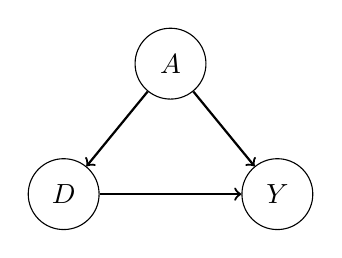
\begin{tikzpicture}[every node/.style={draw, circle, minimum size=9mm, inner sep=1pt}, node distance=18mm]
	\node (D) {$D$};
	\node[right=of D] (Y) {$Y$};
	\node[above=12mm of $(D)!0.5!(Y)$] (A) {$A$};
	\draw[->, thick] (D) -- (Y);
	\draw[->, thick] (A) -- (D);
	\draw[->, thick] (A) -- (Y);
\end{tikzpicture}
\end{center}
\smallskip
{\small $D$ = education, $Y$ = wages, $A$ = ability}
\end{column}
\begin{column}{0.55\textwidth}
\begin{itemize}
	\item Nodes are variables; arrows are direct causal effects; no cycles allowed
	(``acyclic'').

	\item Every \alert{missing arrow is an assumption}: this graph asserts nothing
	else causes both $D$ and $Y$.

	\item Unobserved variables (like ability) still belong in the graph --- being
	unobservable doesn't stop something from causing things.
\end{itemize}
\end{column}
\end{columns}
\end{frame}


\begin{frame}{Paths: how association travels}
In the graph on the last slide there are two paths from $D$ to $Y$:
\begin{enumerate}
	\item $D \rightarrow Y$: the \alert{causal path}. This is the thing we want to measure.
	\item $D \leftarrow A \rightarrow Y$: a \alert{backdoor path}. Association flows
	along it even though $D$ causes none of it.
\end{enumerate}
\bigskip
\begin{itemize}
	\item The regression of $Y$ on $D$ alone picks up \emph{both} paths --- this is
	exactly the omitted variables bias formula from Lecture 2, drawn as a picture.

	\medskip
	\item \alert{Identification strategy = a plan for shutting every backdoor path
	while leaving the causal path alone.}
\end{itemize}
\end{frame}


\begin{frame}{Good controls: closing a backdoor}
\begin{columns}
\begin{column}{0.45\textwidth}
\begin{center}
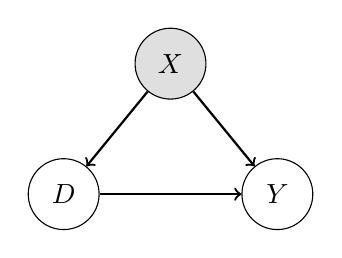
\begin{tikzpicture}[every node/.style={draw, circle, minimum size=9mm, inner sep=1pt}, node distance=18mm]
	\node (D) {$D$};
	\node[right=of D] (Y) {$Y$};
	\node[above=12mm of $(D)!0.5!(Y)$, fill=gray!25] (X) {$X$};
	\draw[->, thick] (D) -- (Y);
	\draw[->, thick] (X) -- (D);
	\draw[->, thick] (X) -- (Y);
\end{tikzpicture}
\end{center}
\smallskip
{\small Shading $=$ conditioned on.}
\end{column}
\begin{column}{0.55\textwidth}
\begin{itemize}
	\item Conditioning on a \alert{confounder} $X$ (regression control, matching,
	stratification) \alert{blocks} the backdoor path $D \leftarrow X \rightarrow Y$.

	\item This is the \alert{backdoor criterion} (informally): find a set of observed
	variables that blocks every backdoor path, condition on them, and the remaining
	association is causal.

	\item ``Selection on observables'' (matching, next month) is exactly the claim
	that such a set exists \emph{and you have it}.
\end{itemize}
\end{column}
\end{columns}
\end{frame}


\begin{frame}{Colliders: conditioning can \emph{open} a path}
\begin{columns}
\begin{column}{0.45\textwidth}
\begin{center}
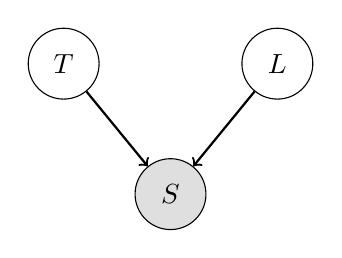
\begin{tikzpicture}[every node/.style={draw, circle, minimum size=9mm, inner sep=1pt}, node distance=18mm]
	\node (D) {$T$};
	\node[right=of D] (Y) {$L$};
	\node[below=12mm of $(D)!0.5!(Y)$, fill=gray!25] (C) {$S$};
	\draw[->, thick] (D) -- (C);
	\draw[->, thick] (Y) -- (C);
\end{tikzpicture}
\end{center}
\smallskip
{\small $T$ = talent, $L$ = luck, $S$ = startup gets funded.}
\end{column}
\begin{column}{0.55\textwidth}
\begin{itemize}
	\item $S$ is a \alert{collider} on the path $T \rightarrow S \leftarrow L$: two
	arrows collide into it. A collider \alert{blocks} the path \emph{by default}.

	\item But \alert{conditioning on a collider opens the path}: among \emph{funded}
	startups, talent and luck are negatively correlated --- if a funded founder wasn't
	talented, they must have been lucky.

	\item Talent and luck are independent in the population. The correlation is
	manufactured by the conditioning. This is \alert{selection bias, drawn as a picture}.
\end{itemize}
\end{column}
\end{columns}
\end{frame}


\begin{frame}{Bad control \#1: the post-treatment variable}
\begin{columns}
\begin{column}{0.45\textwidth}
\begin{center}
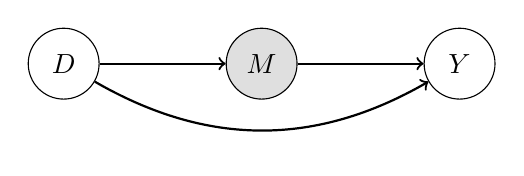
\begin{tikzpicture}[every node/.style={draw, circle, minimum size=9mm, inner sep=1pt}, node distance=16mm]
	\node (D) {$D$};
	\node[right=of D, fill=gray!25] (M) {$M$};
	\node[right=of M] (Y) {$Y$};
	\draw[->, thick] (D) -- (M);
	\draw[->, thick] (M) -- (Y);
	\draw[->, thick] (D) to[bend right=30] (Y);
\end{tikzpicture}
\end{center}
\smallskip
{\small $D$ = education, $M$ = occupation, $Y$ = wages}
\end{column}
\begin{column}{0.55\textwidth}
\begin{itemize}
	\item $M$ is a \alert{mediator}: part of \emph{how} education raises wages is by
	changing occupations.

	\item Controlling for occupation \alert{blocks part of the effect you are trying
	to measure}. The coefficient on $D$ is no longer the total effect.

	\item Rule of thumb with real teeth: \alert{do not control for variables that are
	themselves outcomes of the treatment}. When in doubt, ask: was this variable
	determined before or after $D$?
\end{itemize}
\end{column}
\end{columns}
\end{frame}


\begin{frame}{Bad control \#2: the collider / sample-selection control}
\begin{columns}
\begin{column}{0.45\textwidth}
\begin{center}
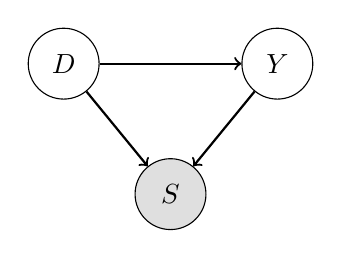
\begin{tikzpicture}[every node/.style={draw, circle, minimum size=9mm, inner sep=1pt}, node distance=16mm]
	\node (D) {$D$};
	\node[right=18mm of D] (Y) {$Y$};
	\node[below=12mm of $(D)!0.5!(Y)$, fill=gray!25] (S) {$S$};
	\draw[->, thick] (D) -- (Y);
	\draw[->, thick] (D) -- (S);
	\draw[->, thick] (Y) -- (S);
\end{tikzpicture}
\end{center}
\smallskip
{\small $D$ = ad exposure, $Y$ = purchase intent, $S$ = visits the site}
\end{column}
\begin{column}{0.55\textwidth}
\begin{itemize}
	\item Estimating the ad effect \alert{only among site visitors} conditions on a
	collider: both seeing the ad and wanting the product cause visits.

	\item Within visitors, exposure and intent are spuriously related even if the ad
	does nothing.

	\item This is the same disease as Heckman's sample selection (Lecture 11) and the
	``conditioning on graduation'' problem in education studies. \alert{Who is in your
	sample, and did the treatment help put them there?}
\end{itemize}
\end{column}
\end{columns}
\end{frame}


\begin{frame}{Case study: when prices respond to your experiment}
\begin{columns}
\begin{column}{0.45\textwidth}
\begin{center}
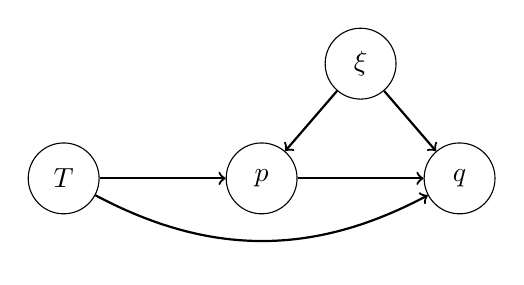
\begin{tikzpicture}[every node/.style={draw, circle, minimum size=9mm, inner sep=1pt}, node distance=16mm]
	\node (T) {$T$};
	\node[right=of T] (P) {$p$};
	\node[right=of P] (Q) {$q$};
	\node[above=10mm of $(P)!0.5!(Q)$] (Xi) {$\xi$};
	\draw[->, thick] (T) -- (P);
	\draw[->, thick] (P) -- (Q);
	\draw[->, thick] (T) to[bend right=28] (Q);
	\draw[->, thick] (Xi) -- (Q);
	\draw[->, thick] (Xi) -- (P);
\end{tikzpicture}
\end{center}
\smallskip
{\small $T$ = randomized ad/feature, $p$ = price, $q$ = quantity, $\xi$ = demand shock (unobserved)}
\end{column}
\begin{column}{0.55\textwidth}
\begin{itemize}
	\item A marketplace A/B test improves product pages. Demand rises --- and
	\alert{treated sellers raise prices}, offsetting part of the sales gain.

	\item Often the estimand is the \alert{direct effect}: the demand-curve shift,
	\emph{holding price constant}.

	\item So this time we \emph{want} to hold the mediator fixed --- but $p$ is a
	\alert{doubly bad control}: post-treatment ($T \rightarrow p$) \emph{and}
	correlated with the demand shock ($\xi \rightarrow p$: sellers reprice when
	demand is hot).
\end{itemize}
\end{column}
\end{columns}
\end{frame}


\begin{frame}{Three regressions, one instrument}
With randomized $T$, positive direct effect, and prices that respond
(Jeziorski, Leng \& Seiler 2025, working paper):
\begin{enumerate}
	\item $q$ on $T$: the \alert{total} effect --- demand shift \emph{minus} the price
	offset. A fine estimand, but it is not the demand shift.

	\item $q$ on $T$ and $p$: \alert{biased for the direct effect even though $T$ is
	randomized} --- $p$ drags $\xi$ into the regression. Typically the bias shrinks
	but does not vanish, and it has the same sign as omitting $p$. The middle answer
	is still a wrong answer.

	\item The fix: a \alert{price instrument} (a cost shifter that moves $p$ but not
	demand) recovers the direct effect. Instruments are next week's topic --- note
	that here the instrument is for the \alert{control}, not the treatment.
\end{enumerate}
\medskip
\begin{itemize}
	\item Built-in diagnostic: regress $p$ on $T$. If price responds to your
	randomized treatment, regressions (1) and (2) answer different questions than
	you think.
	\item Stakes: in supermarket scanner data, not instrumenting price overstates
	feature-advertising effects by a factor of 3--4 in some categories.
	\item You will do all four steps yourself in Assignment 3.
\end{itemize}
\end{frame}


\begin{frame}{The research designs of this course, as DAGs}
\begin{columns}
\begin{column}{0.5\textwidth}
\begin{center}
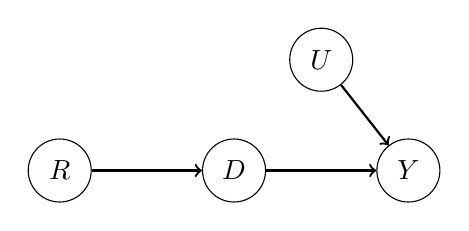
\begin{tikzpicture}[every node/.style={draw, circle, minimum size=8mm, inner sep=1pt}, node distance=14mm]
	\node (R) {$R$};
	\node[right=of R] (D) {$D$};
	\node[right=of D] (Y) {$Y$};
	\node[above=10mm of $(D)!0.5!(Y)$] (U) {$U$};
	\draw[->, thick] (R) -- (D);
	\draw[->, thick] (D) -- (Y);
	\draw[->, thick] (U) -- (Y);
\end{tikzpicture}\\
{\small \alert{Randomization}: coin flip $R$ causes $D$; no arrow into $D$ from $U$.}
\end{center}
\end{column}
\begin{column}{0.5\textwidth}
\begin{center}
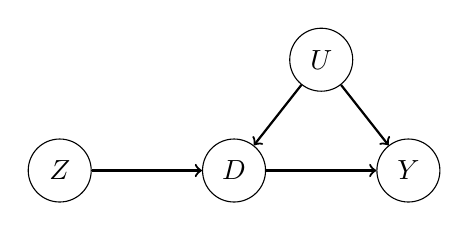
\begin{tikzpicture}[every node/.style={draw, circle, minimum size=8mm, inner sep=1pt}, node distance=14mm]
	\node (Z) {$Z$};
	\node[right=of Z] (D) {$D$};
	\node[right=of D] (Y) {$Y$};
	\node[above=10mm of $(D)!0.5!(Y)$] (U) {$U$};
	\draw[->, thick] (Z) -- (D);
	\draw[->, thick] (D) -- (Y);
	\draw[->, thick] (U) -- (D);
	\draw[->, thick] (U) -- (Y);
\end{tikzpicture}\\
{\small \alert{Instrumental variables}: the missing arrows $Z \rightarrow Y$ (exclusion)
and $U \rightarrow Z$ (exogeneity) ARE the IV assumptions.}
\end{center}
\end{column}
\end{columns}
\bigskip
Every design we meet from here on is a claim about missing arrows. When you referee a
paper, \alert{draw its DAG} --- the contestable assumption is usually an arrow the
authors need to be absent.
\end{frame}


\begin{frame}{Where DAGs strain (and economists push back)}
\begin{itemize}
	\item \alert{Simultaneity}: supply and demand determine price and quantity
	\emph{jointly} --- a cycle, which a DAG cannot draw. Our oldest identification
	problem (Working 1927, Lecture 6) sits awkwardly in this language.

	\medskip
	\item \alert{Heterogeneous effects}: LATE, compliers, and monotonicity
	(Lecture 7) are natural in potential outcomes and clumsy in DAGs.

	\medskip
	\item \alert{Where DAGs shine}: bad controls, sample selection, and transparent
	communication of assumptions --- especially in fields (marketing, IS) where
	``we controlled for everything'' is still treated as a virtue.

	\medskip
	\item Verdict: use the DAG to decide \emph{what to control for}; use potential
	outcomes to decide \emph{what your estimate means}.
\end{itemize}
\end{frame}


\section{When units interfere}

\begin{frame}{The assumption every A/B test makes without saying so}
\begin{itemize}
	\item Everything so far assumed my treatment does not affect \emph{your} outcome. That is the
	\alert{no-interference} half of SUTVA. As a DAG: no arrows between units.
	\medskip
	\item It fails whenever units share something:
	\begin{itemize}
		\item a \alert{market}: a coupon for treated buyers lets them grab inventory control buyers wanted;
		promoting treated sellers diverts demand from control sellers;
		\item a \alert{network}: a feature shown to treated users changes what their control friends see;
		\item a \alert{resource}: discounted rides for treated riders lengthen waits for control riders;
		drivers reallocate toward treated neighborhoods;
		\item \alert{geography or time}: a store-level promotion pulls shoppers from the control store across the street.
	\end{itemize}
	\medskip
	\item When it fails, ``treated minus control'' is not the effect of treating everyone. It is the effect of
	treating \emph{half} the units \emph{while the other half is untreated}, which is an experiment nobody
	plans to run at scale.
\end{itemize}
\end{frame}


\begin{frame}{A marketplace, simulated}
\begin{itemize}
	\item $200$ markets, $200$ buyers each, a shared inventory per market. A buyer wants to purchase with
	probability $0.20$; a \alert{coupon} raises that to $0.30$. Purchases happen in random order until
	inventory runs out.
	\medskip
	\item Three numbers, each with a known truth:
	\begin{itemize}
		\item \alert{Buyer-level A/B}: randomize the coupon across buyers within each market; compare treated
		and control buyers. The experiment every platform runs by default.
		\item \alert{Global treatment effect}: sales per buyer with the coupon for everyone minus sales per buyer
		with it for no one. The number the business decision needs.
		\item \alert{Market-level randomization}: give the coupon to everyone in a random half of the markets.
	\end{itemize}
	\medskip
	\item The one knob: how much inventory there is relative to demand without the coupon.
\end{itemize}
\end{frame}


\begin{frame}{When supply binds, the A/B test measures the wrong thing}
\begin{center}
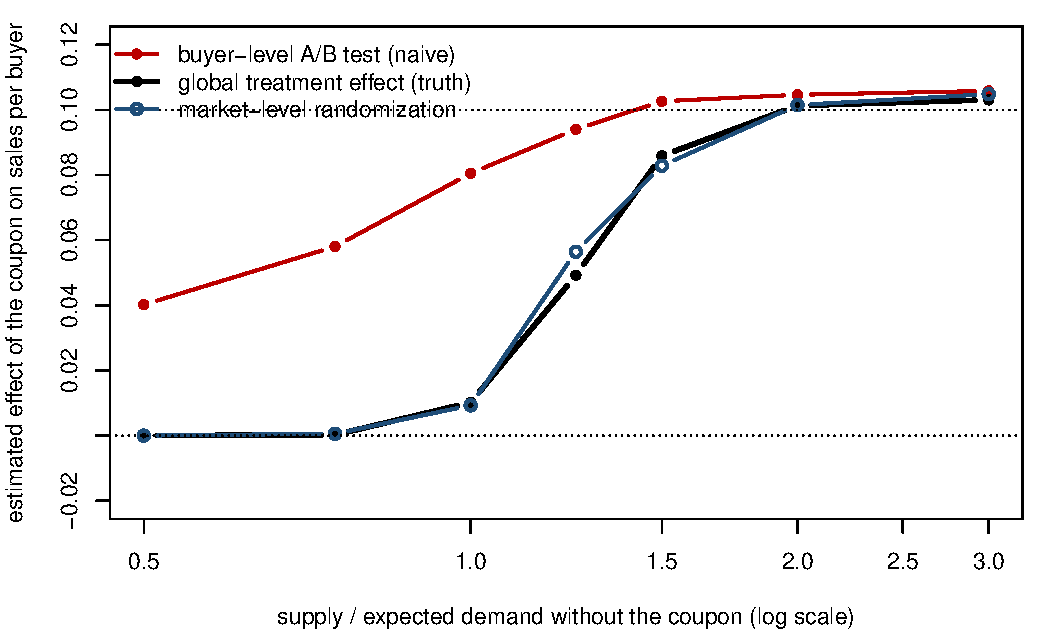
\includegraphics[width=.58\textwidth]{fig_interference.pdf}
\end{center}
\vspace{-.3cm}
{\small With inventory at $75\%$ of demand, the coupon cannot raise total sales at all: the truth is zero.
The buyer-level test reports $+0.06$, because treated buyers took units that control buyers would have bought.
Only when supply is slack do the three numbers agree. Blake and Coey (2014) found exactly this at eBay.}
\end{frame}


\begin{frame}{The same picture as a table}
\begin{center}
\small
\begin{tabular}{lccccc}\toprule
Supply / control demand & Buyer-level A/B & Global effect (truth) & Market-level randomization & SE, buyer-level & SE, market-level \\ \midrule
0.75 & 0.058 & 0.000 & 0.001 & 0.0034 & 0.0003 \\
1.00 & 0.081 & 0.010 & 0.009 & 0.0038 & 0.0016 \\
2.00 & 0.105 & 0.101 & 0.101 & 0.0045 & 0.0045 \\
\bottomrule\end{tabular}

\end{center}
\medskip
\begin{itemize}
	\item The buyer-level test is precise and wrong: a tight standard error around a number that answers no
	business question. A partially binding constraint biases it partway.
	\item Market-level randomization is unbiased for the global effect; its price is precision, since the
	effective sample size is the number of markets. Johari, Li, Liskovich and Weintraub (2022) derive the bias
	in a queueing model and show that randomizing over buyers \emph{and} listings reduces it.
\end{itemize}
\end{frame}


\begin{frame}{Designs that survive interference}
\begin{itemize}
	\item \alert{Cluster randomization.} Randomize at the unit where spillovers stop: markets, cities, stores,
	ego-networks (Saveski et al.\ 2017 at LinkedIn). Estimand: the global effect, if clusters are closed.
	\item \alert{Switchbacks.} One market, treatment on and off in alternating time blocks (DoorDash, Lyft;
	Bojinov, Simchi-Levi and Zhao 2023). For markets you cannot split; needs carryover to die out between blocks.
	\item \alert{Two-sided designs.} Randomize buyers and listings jointly so treated-buyer, treated-listing
	cells exist (Johari et al.\ 2022; Bajari et al.\ 2023 at Amazon).
	\item \alert{Budget-split.} Separate inventories or budgets for treatment and control so they cannot
	compete (ad auctions: Liu et al.\ 2021 at LinkedIn). Removes the interference instead of averaging over it.
	\item \alert{Exposure mapping.} Each unit's treatment is a function of what its neighbors got; estimate
	effects by exposure level (Aronow and Samii 2017). The general framework the others are cases of.
\end{itemize}
\end{frame}


\begin{frame}{What cluster randomization costs: back to power}
\begin{center}
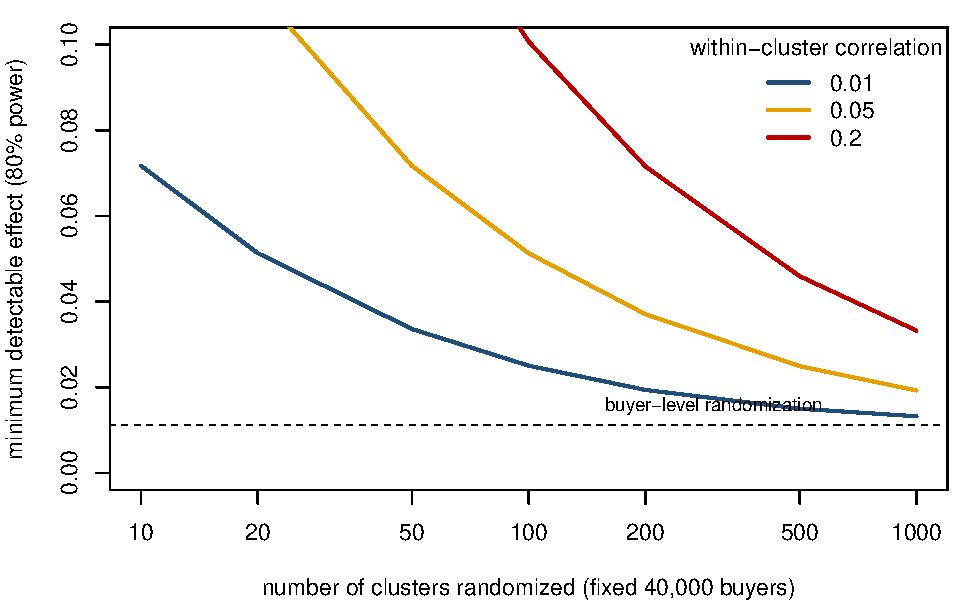
\includegraphics[width=.52\textwidth]{fig_design_effect.pdf}
\end{center}
\vspace{-.3cm}
{\small The design effect $1 + (m - 1)\rho$, with $m$ buyers per cluster and within-cluster correlation $\rho$.
Fixing $40{,}000$ buyers, the minimum detectable effect rises as clusters get fewer and bigger: $50$ metros at
$\rho = 0.05$ detect roughly four times less than buyer-level randomization would. Plan power at the cluster level.}
\end{frame}


\begin{frame}{How to tell whether interference is biting}
\begin{itemize}
	\item \alert{Ask where the outcome comes from.} If treated and control units draw on the same inventory,
	budget, drivers, or attention, assume interference until shown otherwise.
	\medskip
	\item \alert{Run both designs on a small scale.} A buyer-level and a market-level test of the same
	change should agree if there is no interference (Saveski et al.\ 2017 formalize this as a test).
	\medskip
	\item \alert{Vary the treated share.} In a buyer-level test, randomize the \emph{fraction} treated across
	markets ($10\%$, $50\%$, $90\%$). If control buyers' outcomes move with the treated share, they are being
	affected (Hudgens and Halloran 2008).
	\medskip
	\item \alert{Look at the control group's trend.} If control outcomes fall when treatment starts, the
	``effect'' is partly displacement.
	\medskip
	\item \alert{Report which estimand you have.} ``Treated minus control in a $50\%$ buyer-level test'' is a
	fine sentence. ``The effect of the coupon'' is not, unless the design justifies it.
\end{itemize}
\end{frame}



\begin{frame}{Recap}
\begin{itemize}
	\item A DAG is a set of causal assumptions; the missing arrows do the work.
	\item Backdoor paths are confounding; blocking them is what ``controlling for''
	means.
	\item Colliders reverse the logic: conditioning \emph{creates} association.
	Selection into the sample is a collider.
	\item Bad controls: post-treatment variables and colliders. Ask \emph{when} the
	variable was determined and \emph{whether treatment helped put units in the sample}.
	\item Every design in this course is a claim about missing arrows --- draw the
	picture before you believe the number.
\end{itemize}
\end{frame}


\begin{frame}{Workbook time}
\begin{center}
{\LARGE \alert{Let's look at the workbook now.}}
\end{center}
\bigskip
\begin{itemize}
	\item Open \texttt{inclass\_session5.Rmd} (in the \texttt{L7 - Program Evaluation and Selection} folder of the course repo).
	\item Reproduce the power calculations and the funded-startup collider.
	\item Then work the two problems with a neighbor:
	\begin{enumerate}
		\item The bad control, live
		\item Design your own experiment
	\end{enumerate}
\end{itemize}
\end{frame}


\section{Thanks!}

\end{document}
